%!TEX root = ../../book_ML.tex
\chapter{Hồi quy softmax}
\label{cha:softmax}
\index{hồi quy softmax -- softmax regression}
Các bài toán phân loại thực tế thường có nhiều lớp dữ liệu. Như đã thảo luận
trong Chương~\ref{cha:logisticregression}, các bộ phân loại nhị phân tuy có thể
kết hợp với nhau để giải quyết các bài toán phân loại đa lớp nhưng chúng vẫn có
những hạn chế nhất định. Trong chương này, một phương pháp mở rộng của hồi quy
logistic có tên là \textit{hồi quy softmax} sẽ được giới thiệu nhằm khắc phục
những hạn chế đã đề cập. Một lần nữa, mặc dù trong tên có chứa từ ``hồi quy'',
hồi quy softmax được sử dụng cho các bài toán phân loại. Hồi quy softmax là một
trong những thành phần phổ biến nhất trong các bộ phân loại hiện nay.


% % Các bài toán classification thực tế thường có rất nhiều classes (multi-class), các \href{http://machinelearningcoban.com/2017/02/11/binaryclassifiers/#-binary-classifiers-cho-multi-class-classification-problems}{binary classifiers mặc dù có thể áp dụng cho các bài toán multi-class}, chúng vẫn có những hạn chế nhất định. Với binary classifiers, kỹ thuật được sử dụng nhiều nhất \href{http://machinelearningcoban.com/2017/02/11/binaryclassifiers/#one-vs-rest-hay-one-hot-coding}{\textbf{one-vs-rest}} có \href{http://machinelearningcoban.com/2017/02/11/binaryclassifiers/#han-che-cua-one-vs-rest}{một hạn chế về tổng các xác suất}. Trong post này, một phương pháp mở rộng của Logistic Regression sẽ được giới thiệu giúp khắc phục hạn chế trên. Một lần nữa, dù là Softmax \textbf{Regression}, phương pháp này được sử dụng rộng rãi như một phương pháp classification.  
 
 
 
% \textbf{Một lưu ý nhỏ:} Hàm mất mát của Softmax Regression trông có vẻ khá phức tạp, nhưng nếu  kiên trì đọc đến phần phương pháp tối ưu, các bạn sẽ thấy vẻ đẹp ẩn sau sự phức tạp đó. Gradient của hàm mất mát và công thức cập nhật ma trận trọng số là rất đơn giản. (Đơn giản sau vài bước biến đổi toán học \textit{trông có vẻ} phức tạp). 
 
% Nếu có điểm nào khó hiểu, bạn đọc được khuyến khích đọc lại các chương trước, trong đó quan trọng nhất là \href{http://machinelearningcoban.com/2017/01/27/logisticregression/}{Logistic Regression}. 
 
\section{Giới thiệu }

% Với các bài toán phân loại đa lớp, việc 
Với bài toán phân loại nhị phân sử dụng hồi quy logistic, đầu ra của mạng neural
là một số thực trong khoảng $(0, 1)$, có ý nghĩa như xác suất để đầu vào thuộc
một trong hai lớp. Ý tưởng này cũng có thể mở rộng cho bài toán phân loại đa
lớp, ở đó có $C$ nút ở tầng đầu ra và giá trị mỗi nút đóng vai trò như xác
suất để đầu vào rơi vào lớp tương ứng. Như vậy, các đầu ra này liên kết với nhau
qua việc chúng đều là các số dương và có tổng bằng một. Mô hình hồi quy softmax
thảo luận trong chương này đảm bảo tính chất đó.

Nhắc lại biểu diễn dưới dạng mạng neural của kỹ thuật \textit{one-vs-rest} như
trong Hình~\ref{fig:13_1}. Tầng đầu ra có thể tách thành hai \textit{tầng con}
$\bz$ và $\ba$. Mỗi thành phần của tầng con thứ hai $a_i$ chỉ phụ thuộc vào
thành phần tương ứng ở tầng con thứ nhất $z_i$ thông qua hàm sigmoid $a_i =
\sigma(z_i)$. Các giá trị đầu ra $a_i$ đều là các số dương nhưng vì không có
ràng buộc giữa chúng, tổng các xác suất này không đảm bảo bằng một.


% Giả sử có $C$ lớp dữ liệu. Với one-vs-rest, ta cần xây dựng $C$ mô hình
% logistic
% regression khác nhau. Các \textit{đầu ra dự đoán} được tính theo hàm sigmoid
% \begin{equation} 
% a_i = \sigma(z_i) = \sigma(\bx^T\bw_i) 
% \end{equation} 
% Trong kỹ thuật này, các phần tử $a_i, i = 1, 2, \dots, C$ được suy ra trực tiếp
% từ $z_i$. Vì vậy, không có mối quan hệ chặt chẽ nào giữa các $a_i$, tức tổng
% của chúng có thể nhỏ hơn hoặc lớn hơn một. Một cách tự nhiên, nếu ta có thể khai
% thác được mỗi quan hệ giữa các $z_i$ thì kết quả của bài toán phân loại có thể
% được cải thiện. 


% \begin{figure}[t]
%     % caption on side     
   
%     \floatbox[{\capbeside\thisfloatsetup{capbesideposition={right,top},capbesidewidth=4cm}}]{figure}[\FBwidth]
%     {\caption{ 
%     Phân loại đa lớp với hồi quy logistic và one-vs-rest.
%     }
%     \label{fig:13_1}}
%     { % figure here
%     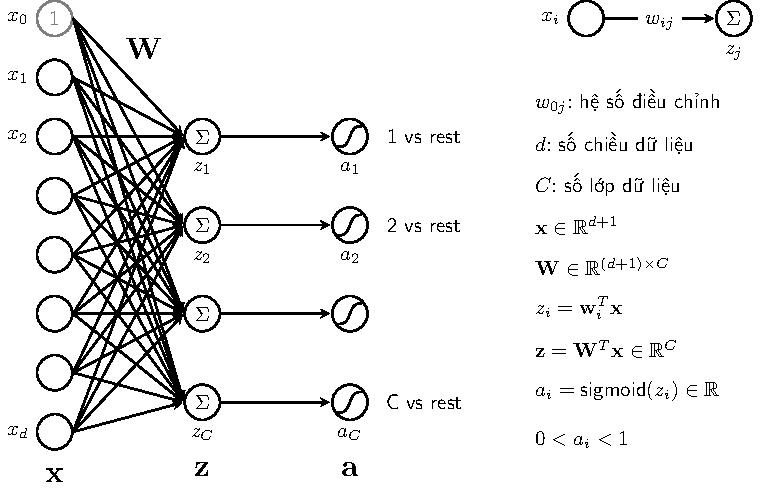
\includegraphics[width=.7\textwidth]{Chapters/05_NeuralNetworks/13_softmax/latex/onevsrest.pdf}
%     }
% \end{figure}
%% *****************************************************************************
\begin{figure}[t]
\centering
    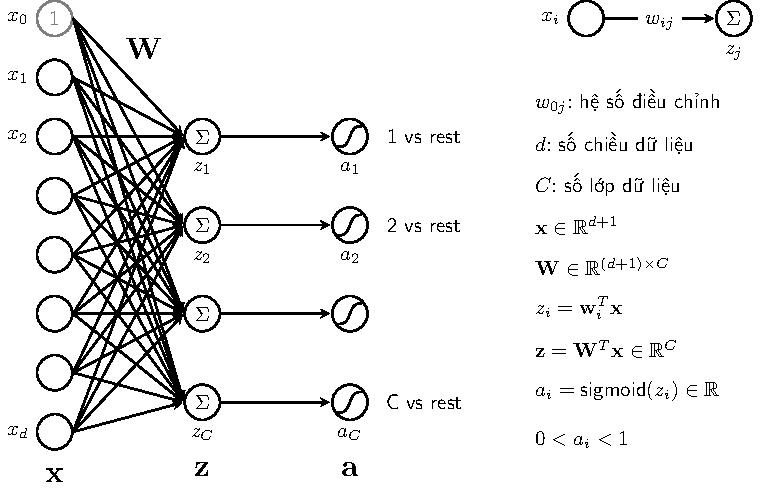
\includegraphics[width =
    .8\textwidth]{Chapters/05_NeuralNetworks/13_softmax/latex/onevsrest.pdf}
    \caption[]{Phân loại đa lớp với hồi quy logistic và one-vs-rest.}
    \label{fig:13_1}
\end{figure}
%% *****************************************************************************
 
% Dữ liệu $\bx$ có số chiều là $(d +1)$ vì có phần tử 1 được thêm vào phía trước, thể hiện hệ số tự do trong hàm tuyến tính. Hệ số tự do $w_{0j}$ còn được gọi là bias.  
 
% Giả sử có $C$ lớp dữ liệu. Với one-vs-rest, ta cần xây dựng $C$ mô hình
% logistic
% regression khác nhau. Các \textit{đầu ra dự đoán} được tính theo hàm sigmoid
% \begin{equation} 
% a_i = \sigma(z_i) = \sigma(\bx^T\bw_i) 
% \end{equation} 
% Trong kỹ thuật này, các phần tử $a_i, i = 1, 2, \dots, C$ được suy ra trực tiếp
% từ $z_i$. Vì vậy, không có mối quan hệ chặt chẽ nào giữa các $a_i$, tức tổng
% của chúng có thể nhỏ hơn hoặc lớn hơn một. Một cách tự nhiên, nếu ta có thể khai
% thác được mỗi quan hệ giữa các $z_i$ thì kết quả của bài toán phân loại có thể
% được cải thiện. 

 
\index{ma trận trọng số -- weight matrix}
Các mô hình hồi quy tuyến tính, PLA, và hồi quy logistic chỉ có một nút ở tầng
đầu ra. Trong các trường hợp đó, tham số mô hình chỉ là một vector $\bw$.
Trong trường hợp tầng đầu ra có nhiều hơn một nút, tham số mô hình sẽ là tập hợp
tham số $\bw_i$ ứng với từng nút. Lúc này, ta có một \textit{ma trận
trọng số} $\bW = [\bw_1, \bw_2, \dots, \bw_C]$, mỗi
cột ứng với một nút ở tầng đầu ra.
 
 
\section{Hàm softmax}
\subsection{Hàm softmax}

Chúng ta cần một mô hình xác suất sao cho với mỗi đầu vào $\bx$, $a_i$ thể hiện
xác suất để đầu vào đó rơi vào lớp thứ $i$. Vậy điều kiện cần là các $a_i$ phải
dương và tổng của chúng bằng một. Ngoài ra, ta sẽ thêm điều kiện giá trị $z_i =
\bx^T\bw_i$ càng lớn thì xác suất dữ liệu rơi vào lớp thứ $i$ càng cao. Điều
kiện cuối này chỉ ra rằng ta cần một quan hệ đồng biến.
 
\index{hàm softmax} 
Chú ý rằng $z_i$ có thể nhận giá trị cả âm và dương vì nó là một tổ hợp tuyến
tính các thành phần của vector đặc trưng $\bx$. Một hàm số khả vi đồng biến đơn
giản có thể biến $z_i $ thành một giá trị dương là hàm $\exp(z_i) = e^{z_i}$.
Hàm số này không những khả vi mà còn có đạo hàm bằng chính nó, việc này mang
lại nhiều lợi ích khi tối ưu. Điều kiện tổng các $a_i$ bằng một có
thể được đảm bảo nếu \begin{equation} a_i = \frac{\exp(z_i)}{\sum_{j=1}^C
\exp(z_j)}, ~~ \forall i = 1, 2, \dots, C.
\end{equation} 
Mối quan hệ này thoả mãn tất cả các điều kiện đã xét: các đầu ra $a_i$ dương, có
tổng bằng một và giữ được {thứ tự} của $z_i$. Hàm số này được gọi là
\textit{hàm softmax}. Lúc này, ta có thể coi rằng 
\begin{equation} 
p(y_k = i | \bx_k; \bW) = a_i 
\end{equation} 
Trong đó, $p(y = i | \bx; \bW)$ được hiểu là xác suất để một điểm
dữ liệu $\bx$ rơi vào lớp thứ $i$ nếu biết tham số mô hình là ma trận
trọng số $\bW$.  
Hình~\ref{fig:13_2} thể hiện mô hình hồi quy softmax dưới dạng mạng neural. Mô hình này khác one-vs-rest nằm ở chỗ nó có các liên kết giữa mọi nút của hai tầng con $\bz$ và $\ba$. 

% <div class="imgcap"> 
% <img src ="\assets\13_softmax\softmax_nn.png" align = "center" width = "800"> 
% <div class = "thecap">Hình 2: Mô hình Softmax Regression dưới dạng Neural network.</div> 
% </div>  
% \begin{figure}[t]
%     % caption on side     
   
%     \floatbox[{\capbeside\thisfloatsetup{capbesideposition={right,top},capbesidewidth=4cm}}]{figure}[\FBwidth]
%     {\caption{ 
%     Mô hình hồi quy softmax dưới dạng neural network.
%     }
%     \label{fig:13_2}}
%     { % figure here
%     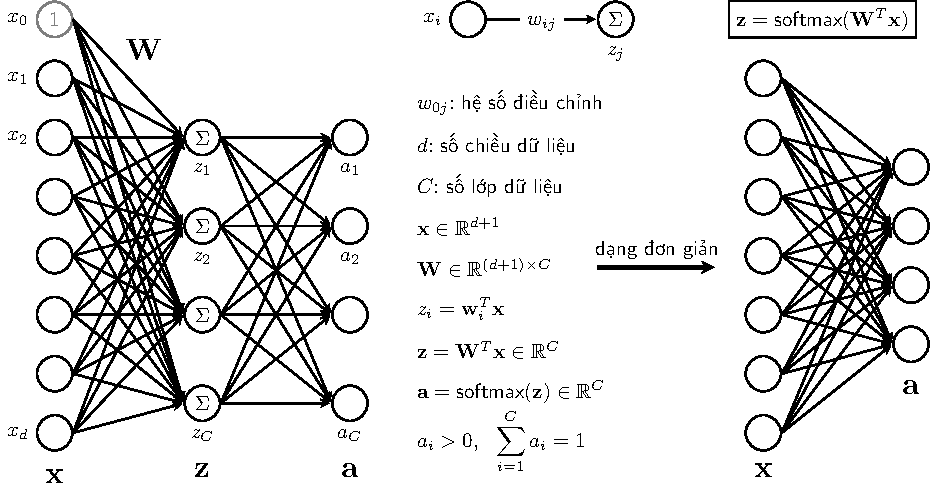
\includegraphics[width=.7\textwidth]{Chapters/05_NeuralNetworks/13_softmax/latex/softmax_nn.pdf}
%     }
% \end{figure}

%% *****************************************************************************
\begin{figure}[t]
\centering
    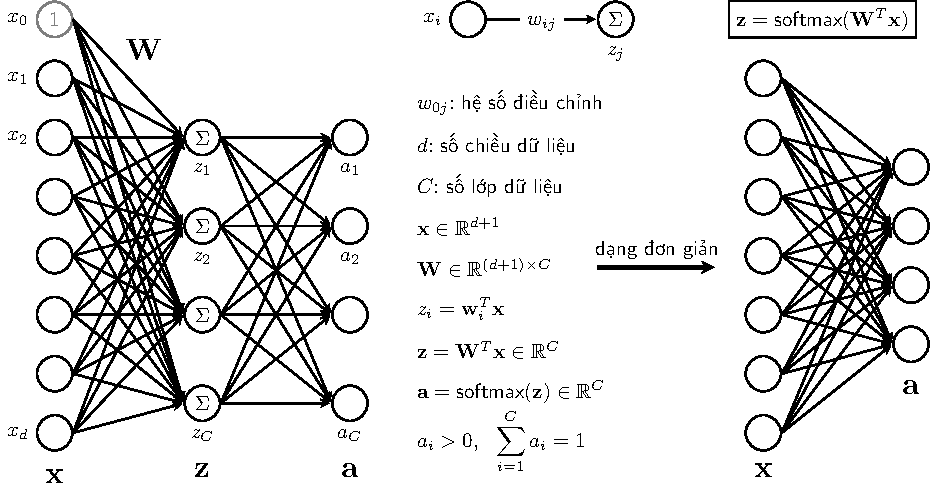
\includegraphics[width =
    .9\textwidth]{Chapters/05_NeuralNetworks/13_softmax/latex/softmax_nn.pdf}
    \caption[]{Mô hình hồi quy softmax dưới dạng neural network.}
    \label{fig:13_2}
\end{figure}
%% *****************************************************************************

% Ở phần bên phải, hàm tuyến tính $\Sigma$ và hàm softmax (activation function) được tách riêng ra để phục vụ cho mục đích minh họa. Dạng \textit{short form} ở bên phải là dạng hay được sử dụng trong các Neural Networks, lớp $\mathbf{a}$ được ngầm hiểu là bao gồm cả lớp $\mathbf{z}$. 
 
 
 
 
\subsection{Xây dựng hàm softmax trong Python }
Dưới đây là một đoạn code thực hiện hàm softmax. Đầu vào là một ma trận với mỗi
\textit{hàng} là một vector $\mathbf{z}$, đầu ra cũng là một ma trận mà mỗi hàng có
giá
trị là $\mathbf{a} = \text{softmax}(\mathbf{z})$. Các giá trị của $\mathbf{z}$ còn được gọi là \textit{score}:
 
\begin{lstlisting}[language=Python]
import numpy as np  
def softmax(Z):
    """
    Compute softmax values for each sets of scores in Z.
    each column of Z is a set of scores.    
    Z: a numpy array of shape (N, C)
    return a numpy array of shape (N, C)
    """
    e_Z = np.exp(Z)
    A = e_Z / e_Z.sum(axis = 1, keepdims = True)
    return A
\end{lstlisting}
 
 
\subsection{Một vài ví dụ }
 
Hình~\ref{fig:13_3} mô tả một vài ví dụ về mối quan hệ giữa đầu vào và đầu ra
của hàm softmax. Hàng trên thể hiện các score $z_i$ với giả sử rằng số lớp dữ
liệu là ba. Hàng dưới thể hiện các giá trị đầu ra $a_i$ của hàm softmax.
 
% \begin{figure}[t]
%     % caption on side     
%     \floatbox[{\capbeside\thisfloatsetup{capbesideposition={right,top},capbesidewidth=6cm}}]{figure}[\FBwidth]
%     {\caption{ 
%     Một số ví dụ về đầu vào và đầu ra của hàm softmax.
%     }
%     \label{fig:13_3}}
%     { % figure here
%     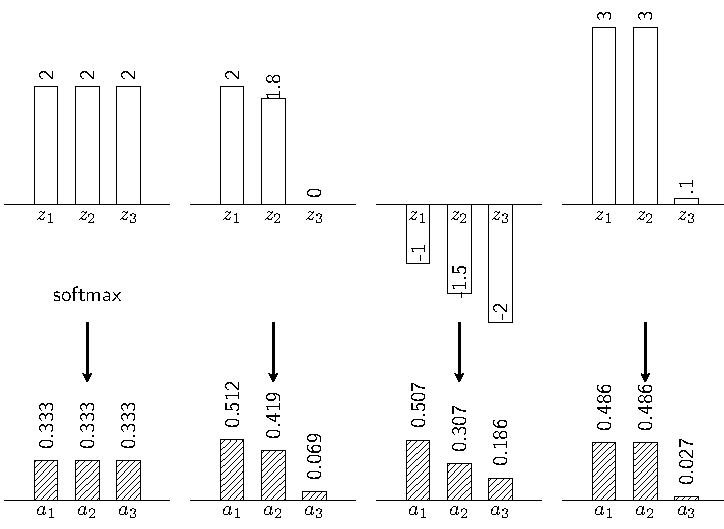
\includegraphics[width=.5\textwidth]{Chapters/05_NeuralNetworks/13_softmax/latex/softmax_ex.pdf}
%     }
% \end{figure}

%% *****************************************************************************
\begin{figure}[t]
\centering
    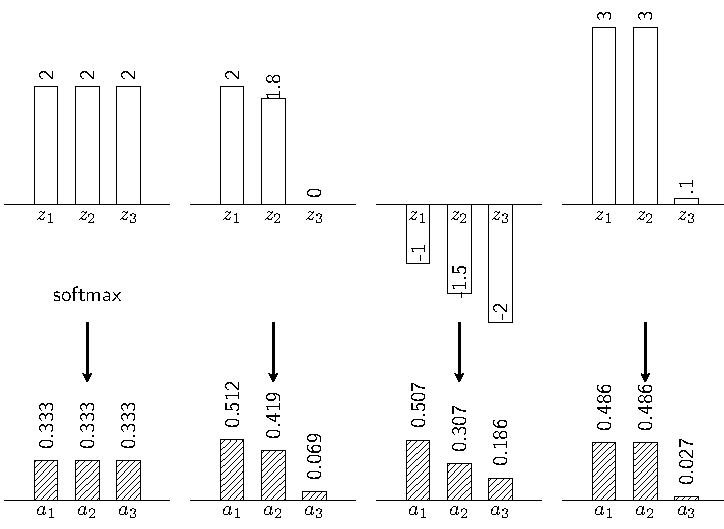
\includegraphics[width =
    .8\textwidth]{Chapters/05_NeuralNetworks/13_softmax/latex/softmax_ex.pdf}
    \caption[]{Một số ví dụ về đầu vào và đầu ra của hàm softmax.}
    \label{fig:13_3}
\end{figure}
%% *****************************************************************************
 \newpage 
Có một vài quan sát như sau:  
\begin{itemize}
\item Cột 1: Nếu các $z_i$ bằng nhau (bằng 2 hoặc một số bất kỳ) thì các $a_i$
cũng bằng nhau
và bằng 1/3.
 
\item Cột 2: Nếu giá trị lớn nhất trong các $z_i$ là $z_1$ vẫn bằng 2, thì mặc
dù xác suất
tương ứng $a_1$ vẫn là lớn nhất, nó đã tăng lên hơn 0.5. Sự chênh lệch ở
đầu ra là đáng kể, nhưng thứ tự tương ứng không thay đổi. 

\item Cột 3: Khi các giá trị $z_i$ là âm thì các giá trị $a_i$ vẫn là dương và thứ tự vẫn được đảm bảo.  
 
\item Cột 4: Nếu $z_1 = z_2$ thì $a_1 = a_2$. 
\end{itemize}
 
Bạn đọc có thể thử với các giá trị khác trên trình duyệt tại
\url{https://goo.gl/pKxQYc}, phần softmax.
 
 
\subsection{Phiên bản ổn định hơn của hàm softmax}
 Khi một trong các $z_i$ quá lớn, việc tính toán $\exp(z_i)$ có thể gây ra hiện
tượng tràn số, ảnh hưởng lớn tới kết quả của hàm
softmax. Có một cách khắc phục hiện tượng này dựa trên quan sát
\begin{equation} 
\frac{\exp(z_i)}{\sum_{j=1}^C \exp(z_j)} = \frac{\exp(-c)\exp(z_i)}{\exp(-c)\sum_{j=1}^C \exp(z_j)}\\\ 
= \frac{\exp(z_i-c)}{\sum_{j=1}^C \exp(z_j-c)} 
\end{equation} 
với $c$ là một hằng số bất kỳ. Từ đây, một kỹ thuật đơn giản giúp khắc phục hiện
tượng tràn số là trừ tất cả các $z_i$ đi một giá trị đủ lớn. Trong thực nghiệm,
giá trị đủ lớn này thường được chọn là $c = \max_i z_i$. Ta có thể cải tiến
đoạn code cho hàm \pythoninline{softmax} phía trên bằng cách trừ mỗi hàng của
ma trận đầu vào \pythoninline{Z} đi giá trị lớn nhất trong hàng đó. Ta có phiên
bản ổn định hơn là \pythoninline{softmax_stable}\footnote{Xem thêm về
cách xử lý mảng numpy trong Python tại \url{https://fundaml.com}}:
\begin{lstlisting}[language=Python]
def softmax_stable(Z):
    """
    Compute softmax values for each set of scores in Z.
    each row of Z is a set of scores.    
    """
    e_Z = np.exp(Z - np.max(Z, axis = 1, keepdims = True))
    A = e_Z / e_Z.sum(axis = 1, keepdims = True)
    return A
\end{lstlisting}
% trong đó \pythoninline{axis = 1} nghĩa là hàm \pythoninline{np.max} được áp dụng
% lên mỗi hàng, \pythoninline{keepdims = True} để đảm bảo phép trừ/chia giữa mảng
% hai chiều \pythoninline{Z} và mảng một chiều thực hiện được}.
 
 
 
 
 
 
\section{Hàm mất mát và phương pháp tối ưu }
 
 
\subsection{Entropy chéo}
\index{entropy chéo -- cross entropy}
% Với cách biểu diễn network như trên, mỗi output nút sẽ không còn là một giá trị
% tương ứng với mỗi lớp nữa mà sẽ là một vector có đúng một phần tử bằng một, các
% phần tử còn lại bằng 0. Phần tử bằng 1 năm ở vị trí tương ứng với class đó, thể hiện rằng điểm dữ liệu đang xét rơi vào class này với xác suất bằng 1 (\textit{sự thật} là như thế, không cần dự đoán). Cách \textit{mã hóa} output này chính là \textit{one-hot coding} mà tôi đã đề cập trong bài \href{http://machinelearningcoban.com/2017/01/01/kmeans/}{K-means clustering} và \href{http://machinelearningcoban.com/2017/02/11/binaryclassifiers/#one-vs-rest-hay-one-hot-coding}{bài trước}.
% \tcb{stophere}
\index{one-hot}

\def\softmax{\text{softmax}}
Đầu ra của mạng softmax, $\ba = \softmax(\bW^T\bx)$, là một vector có số phần tử bằng số lớp dữ liệu. Các phần tử của vector này là các số dương có tổng bằng một, thể hiện xác suất để điểm đầu vào rơi vào từng lớp dữ liệu. Với một điểm dữ liệu huấn luyện thuộc lớp thứ $c$, chúng ta mong muốn xác suất tương ứng với lớp này càng cao càng tốt, tức càng gần một càng tốt. Việc này kéo theo các phần tử còn lại gần với không. Một cách tự nhiên, đầu ra thực sự $\by$ là một vector có tất cả các phần tử bằng không trừ phần từ ở vị trí thứ $c$ bằng một. Cách biểu diễn nhãn dưới dạng vector này được gọi là mã hoá \textit{one-hot}. 


Hàm mất mát của hồi quy softmax được xây dựng dựa trên bài toán tối thiểu sự
khác nhau giữa {đầu ra dự đoán} $\mathbf{a}$ và {đầu ra thực sự}
$\mathbf{y}$ ở dạng one-hot. Khi cả hai là các vector thể hiện xác suất,
khoảng cách giữa chúng thường được đo bằng một hàm số được gọi là
\textit{entropy chéo} $H(\by, \ba)$. Đặc điểm nổi bật của hàm số 

Một đặc điểm nổi bật là nếu cố định $\by$, hàm số sẽ đạt giá trị nhỏ nhất khi $\ba = \by$, và càng lớn nếu $\ba$ càng khác $\by$.

% % \subsection{} 
% \begin{equation} 
% J(\bW) = \sum_{i=1}^N \|\mathbf{a}_i - \mathbf{y}_i\|_2^2 
% \end{equation} 

% \textbf{Tuy nhiên đây chưa phải là một lựa chọn tốt}. Khi đánh giá sự khác nhau (hay khoảng cách) giữa hai phân bố xác suất (probability distributions), chúng ta có một đại lượng đo đếm khác hiệu quả hơn. Đại lượng đó có tên là \href{https://en.wikipedia.org/wiki/Cross_entropy}{\textbf{entropy chéo}}. 
 
%%%%%%% Three subfigures with bottom caption%%%%%%%%%%%%%%
\begin{figure}[t]
    \begin{subfigure}{0.325\textwidth}
    % 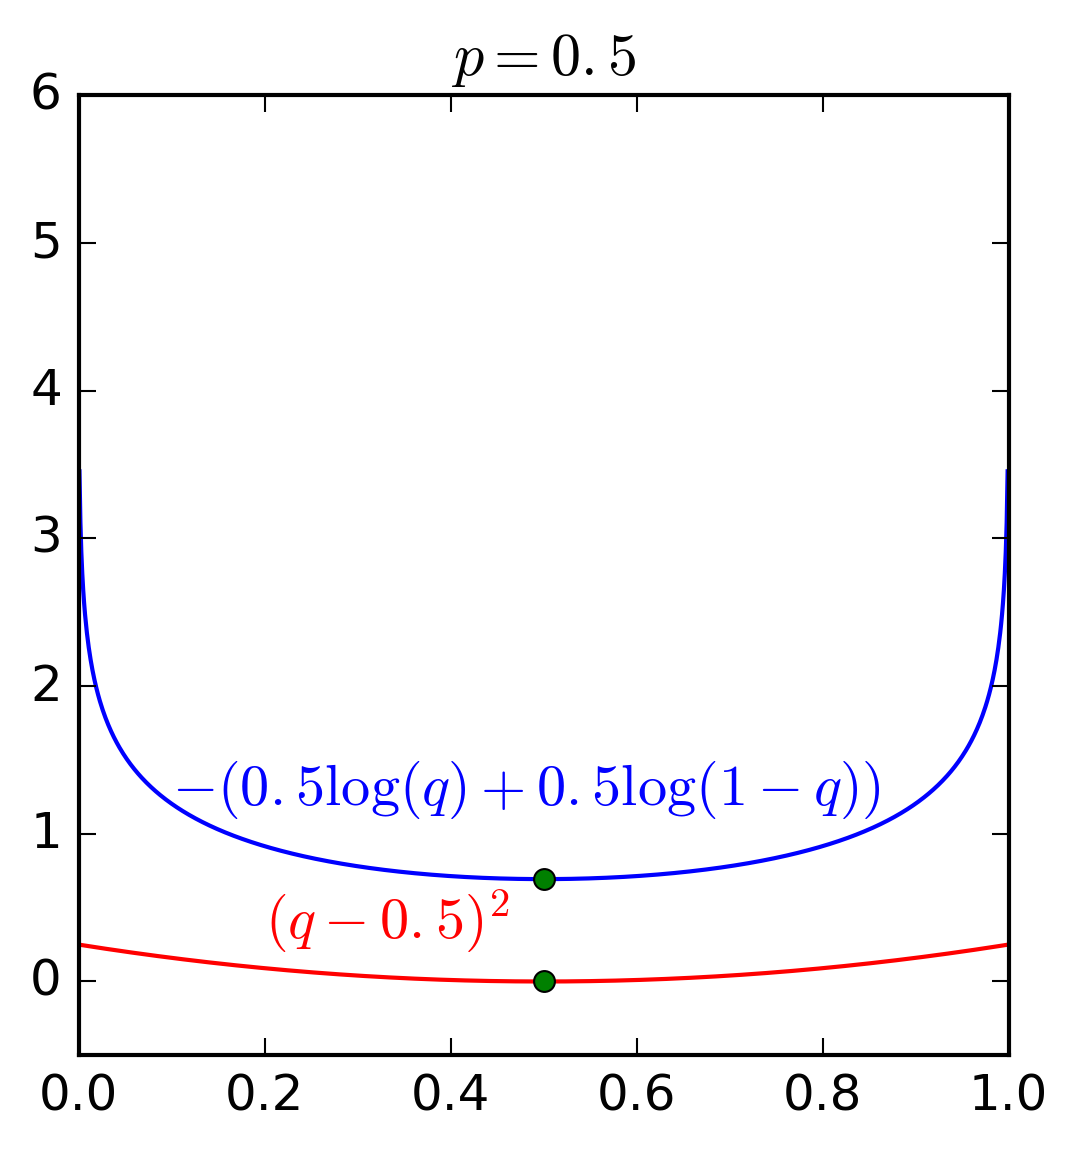
\includegraphics[width=0.99\linewidth]{Chapters/05_NeuralNetworks/13_softmax/crossentropy1.png}
    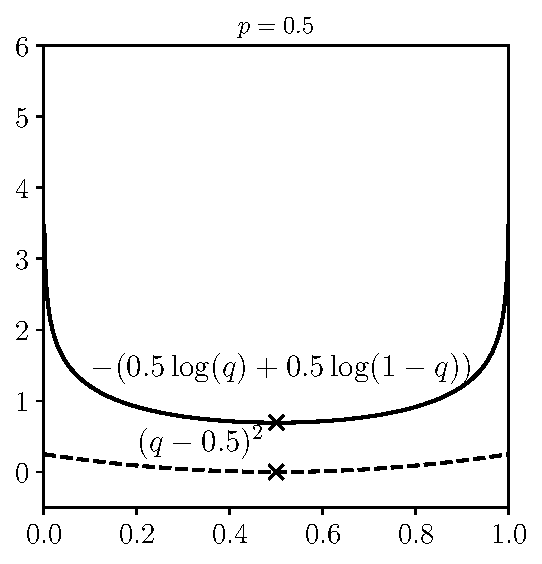
\includegraphics[width=0.99\linewidth]{Chapters/05_NeuralNetworks/13_softmax/crossentropy1.pdf}
    \caption{}
    % \label{fig:subim1}
    \end{subfigure}
    \begin{subfigure}{0.325\textwidth}
    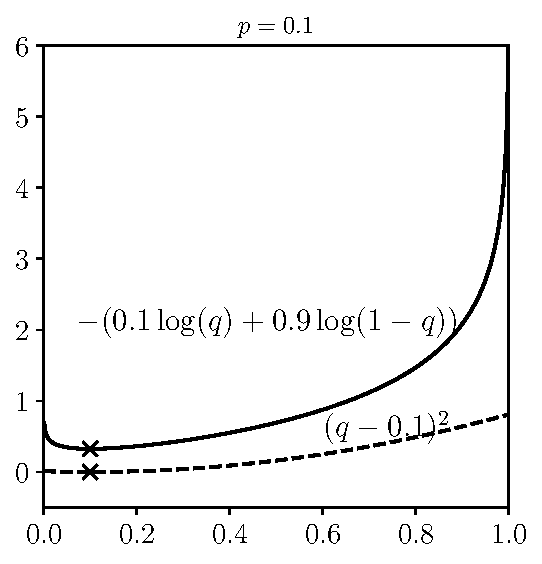
\includegraphics[width=0.99\linewidth]{Chapters/05_NeuralNetworks/13_softmax/crossentropy2.pdf}
    \caption{}
    % \label{fig:subim2}
    \end{subfigure}
    \begin{subfigure}{0.325\textwidth}
    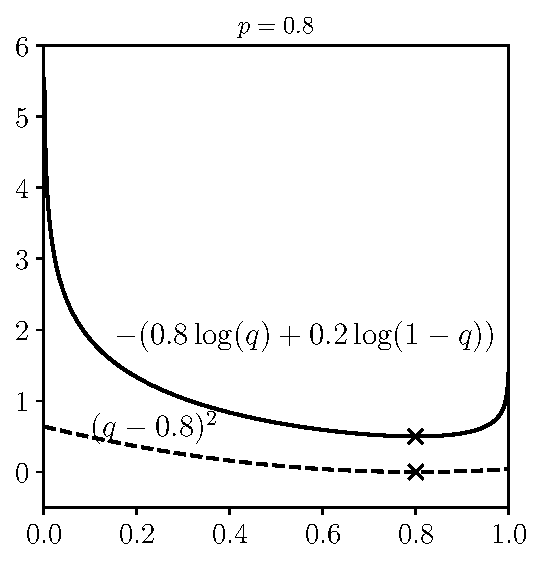
\includegraphics[width=0.99\linewidth]{Chapters/05_NeuralNetworks/13_softmax/crossentropy3.pdf}
    \caption{}
    % \label{fig:subim2}
    \end{subfigure}

    \caption{
    So sánh hàm entropy chéo (đường nét liền) và hàm bình phương khoảng cách
    (đường nét đứt). Các điểm được đánh dấu thể hiện điểm cực tiểu toàn cục
    của mỗi hàm. Càng xa điểm cực tiểu toàn cục, khoảng cách giữa hai hàm số
    càng lớn. }
    \label{fig:13_4}
\end{figure}
% \subsection{Cross Entropy }
Entropy chéo giữa hai vector phân phối $\mathbf{p}$ và $\mathbf{q}$ rời rạc 
được định nghĩa bởi 
\begin{equation} 
\label{eqn:13_1}
H(\mathbf{p}, \mathbf{q}) =-\sum_{i=1}^C p_i \log q_i
\end{equation} 
Hình~\ref{fig:13_4} thể hiện ưu điểm của hàm entropy chéo so với hàm bình
phương khoảng cách Euclid. Đây là ví dụ trong trường hợp $C = 2$ và $p_1$ lần
lượt nhận các giá trị $0.5, 0.1$ và $0.8$ và $p_2 = 1 - p_1$.
Có hai nhận xét quan trọng:
\begin{itemize}
\item Giá trị nhỏ nhất của cả hai hàm số đạt được khi $q = p$ tại hoành độ các điểm được đánh dấu. 
 
\item Nhận thấy rằng hàm entropy chéo nhận giá trị rất cao, tức mất mát rất
cao, khi $q$ ở xa $p$. Sự chênh lệch giữa các mất mát ở gần hay xa
nghiệm của hàm bình phương khoảng cách $(q - p)^2$ là ít đáng kể hơn. Về mặt tối
ưu, hàm entropy chéo sẽ cho nghiệm {gần} với $p$ hơn vì những nghiệm ở xa gây ra mất mát lớn.
\end{itemize}
 
Hai tính chất trên đây khiến hàm entropy chéo được sử dụng rộng rãi khi tính
khoảng cách giữa hai phân phối xác suất. Tiếp theo, chúng ta sẽ chứng minh nhận
định sau. 

\textit{Cho $\bp \in \R_{+}^C$ là một vector với các thành phần dương có tổng
bằng một. Bài toán tối ưu}
\begin{align*}
    \bq &= \arg\min_{\bq} H(\bp, \bq) \\
    \text{thoả mãn:}~&\sum_{i=1}^C q_i = 1; q_i > 0
\end{align*}
\textit{có nghiệm $\bq = \bp$.}

Bài toán này có thể giải quyết bằng phương pháp nhân tử Lagrange (xem Phụ
lục~\ref{apd:lagrange}). 

Lagrangian của bài toán tối ưu này là 
\begin{equation*} 
\mathcal{L}(q_1, q_2, \dots, q_C, \lambda) = -\sum_{i=1}^C p_i \log(q_i) +
\lambda(\sum_{i=1}^C q_i - 1) 
\end{equation*} 
Ta cần giải hệ phương trình
\begin{equation*} 
\nabla_{q_1, \dots, q_C, \lambda} \mathcal{L}(q_1, \dots, q_C, \lambda) = 0
\Leftrightarrow 
\left\{ 
\begin{matrix} 
   -\frac{p_i}{q_i} + \lambda = 0, ~~ i = 1, \dots, C\\\ 
   q_1 + q_2 + \dots + q_C =1 
\end{matrix} 
\right. 
\end{equation*} 
Từ phương trình thứ nhất ta có $p_i = \lambda q_i$. Vì vậy, $ 1 = \sum_{i=1}^C
p_i = \lambda\sum_{i=1}^C q_i = \lambda \Rightarrow \lambda = 1$. Điều này
tương đương với $ q_i
= p_i, \forall i$. \dpcm
 
% Qua đây, chúng ta đã hiểu rằng vì sao hàm số entropy chéo được dùng để \textit{ép} hai xác suất \textit{gần nhau}. 



\begin{mydeff}
\begin{enumerate}
    \item Hàm entropy chéo không có tính đối xứng $H(\mathbf{p},
    \mathbf{q}) \neq H(\mathbf{q}, \mathbf{p})$. Điều này có thể nhận ra 
    từ việc các thành phần của $\mathbf{p}$ trong công thức~\eqref{eqn:13_1} có
    thể nhận giá trị bằng không, trong khi các thành phần của $\mathbf{q}$ phải
    là dương vì $\log(0)$ không xác định. Chính vì vậy, khi sử dụng entropy chéo
    trong các bài toán phân loại, $\mathbf{p}$ là \textit{đầu ra thực sự} ở dang
    one-hot, $\mathbf{q}$ là \textit{đầu ra dự đoán}. Trong các thành phần thể
    hiện xác suất của $\mathbf{q}$, không có thành phần nào tuyệt đối bằng một
    hoặc tuyệt đối bằng không do hàm $\exp$ luôn trả về một giá trị dương.

    \item Khi $\bp$ là một vector ở dạng one-hot, giả sử chỉ có $p_c = 1$, biểu thức entropy chéo trở thành $-\log(q_c)$. Biểu thức này đạt giá trị
    nhỏ nhất nếu $q_c = 1$, điều này không xảy ra vì nghiệm này không thuộc miền
    xác định của bài toán. Tuy nhiên, giá trị entropy chéo tiệm cận tới không
    khi $q_c$ tiến đến một, tức $z_c$ rất rất lớn so với các $z_i$ còn lại.
\end{enumerate}
\end{mydeff}
 
% Trong hồi quy logistic, ta cũng có hai phân phối đơn giản. (i) \textit{Đầu ra
% thực sự} của điểm dữ liệu đầu vào $\bx_i$ có phân phối xác suất là $[y_i;
% 1 - y_i]$ với $y_i$ là xác suất để điểm dữ liệu đầu vào rơi vào class thứ nhất
% (bằng 1 nếu $y_i = 1$, bằng 0 nếu $y_i = 0$). (ii). \textit{Đầu ra dự đoán} của
% điểm dữ liệu đó là $a_i = \text{sigmoid}(\bw^T\bx)$ là xác suất để
% điểm đó rơi vào class thứ nhất. Xác suất để điểm đó rơi vào class thứ hai có thể được dễ dàng suy ra là $1 - a_i$. Vì vậy, hàm mất mát trong hồi quy logistic
% \begin{equation} 
% J(\bw) = -\frac{1}{N}\sum_{i=1}^N(y_i \log {a}_i + (1-y_i) \log (1 -
% {a}_i))
% \end{equation} 
% chính là một trường hợp đặc biệt của entropy chéo. 
\subsection{Xây dựng hàm mất mát} 
Trong trường hợp có $C$ lớp dữ liệu, {mất mát} giữa
đầu ra dự đoán và đầu ra thực sự của một điểm dữ liệu $\bx_i$ với
nhãn $\by_i$ được tính bởi
\begin{equation} 
\label{eqn:13_cross0}
J_i(\bW) \triangleq J(\bW;\bx_i, \mathbf{y}_i) = -\sum_{j=1}^C
y_{ji}\log(a_{ji})
\end{equation} 
với $y_{ji}$ và $ a_{ji}$ lần lượt là phần tử thứ $j$ của vector xác suất
$\mathbf{y}_i$ và $\mathbf{a}_i$. Nhắc lại rằng đầu ra $\mathbf{a}_i$ phụ thuộc vào đầu vào $\bx_i$ và ma trận trọng số $\bW$. 
Tới đây, nếu để ý rằng chỉ có đúng một $j$ sao cho $y_{ji} = 1, \forall i$, biểu
thức~\eqref{eqn:13_cross0} chỉ còn lại một số hạng tương ứng với giá trị $j$ đó.
Để tránh việc sử dụng quá nhiều ký hiệu, chúng ta giả sử rằng $y_i$ là nhãn
của điểm dữ liệu $\bx_i$ (các nhãn là các số tự nhiên từ 1 tới $C$), khi đó $j$
chính bằng $y_i$. Sau khi có
ký hiệu này, ta có thể viết lại
\begin{equation}
    J_i(\bW) = - \log(a_{y_i, i})
\end{equation}
với $a_{y_i, i}$ là phần tử thứ $y_i$ của vector $\ba_i$.

Khi sử dụng toàn bộ tập huấn luyện $\bx_i, \mathbf{y}_i, i = 1, 2, \dots, N$,
hàm mất mát của hồi quy softmax được xác định bởi
\begin{equation} 
\label{eqn:13_loss}
J(\bW; \mathbf{X}, \mathbf{Y}) = -\frac{1}{N}\sum_{i = 1}^N
\log(a_{y_i,i})
% = -\frac{1}{N}\sum_{i = 1}^N 
% \log\left(\frac{\exp(\bw_{y_j}^T\bx_i)}{\sum_{k=1}^C
% \exp(\bx_i^T\bw_k)}\right) 
\end{equation} 
Ở đây, ma trận trọng số $\bW$ là biến cần tối ưu. Hàm mất mát này có gradient khá
gọn, kỹ thuật tính gradient gần giống với hồi quy logistic. Để tránh quá khớp, ta cũng có thể sử dụng cơ chế kiểm soát suy giảm trọng số:
\index{suy giảm trọng số -- weight decay}
\begin{equation}
\label{eqn:13_regloss}
     \bar{J}(\bW; \mathbf{X}, \mathbf{Y}) =
     -\frac{1}{N}\left(\sum_{i = 1}^N \log(a_{y_i,i}) + \frac{\lambda}{2} \|\bW\|_F^2 \right)
 \end{equation}
Trong các mục tiếp theo, chúng ta sẽ làm việc với hàm mất
mát~\eqref{eqn:13_loss}. Việc mở rộng cho hàm mất mát với
cơ chế kiểm soát~\eqref{eqn:13_regloss} không phức tạp vì gradient của số hạng
kiểm soát $\frac{\lambda}{2}\|\bW\|_F^2$ đơn giản là $\lambda \bW$. Hàm mất
mát~\eqref{eqn:13_loss} có thể được thực hiện trên Python như sau\footnote{{Truy cập vào nhiều phần tử của mảng hai
chiều trong numpy - FundaML} \url{https://goo.gl/SzLDxa}.}:
\begin{lstlisting}[language=Python]
def softmax_loss(X, y, W):
    """
    W: 2d numpy array of shape (d, C), 
        each column correspoding to one output node
    X: 2d numpy array of shape (N, d), each row is one data point
    y: 1d numpy array  --  label of each row of X 
    """
    A = softmax_stable(X.dot(W))
    id0 = range(X.shape[0]) # indexes in axis 0, indexes in axis 1 are in y
    return -np.mean(np.log(A[id0, y]))
\end{lstlisting}

\begin{mydeff}
\begin{enumerate}
    \item Khi biểu diễn dưới dạng toán học, mỗi điểm dữ liệu là một cột của ma trận
    $\bX$; nhưng khi làm việc với numpy, mỗi điểm dữ liệu được đọc theo
    \pythoninline{axis = 0} của mảng hai chiều \pythoninline{X}.
    Việc này
    thống nhất với các thư viện scikit-learn hay tensorflow ở việc
    \pythoninline{X[i]} được dùng để chỉ điểm dữ liệu thứ \pythoninline{i}, tính
    từ \pythoninline{0}. Tức là, nếu có $N$ điểm dữ liệu trong không gian $d$
    chiều thì $\bX \in \R^{d \times N}$, nhưng \pythoninline{X.shape == (N, d)}.

    \item $\bW \in \R^{d\times C}$, \pythoninline{W.shape == (d, C)}. 

    \item $\bW^T\bX$ sẽ được biểu diễn bởi \pythoninline{X.dot(W)}, và có
    \pythoninline{shape == (N, C)}. 

    \item Khi làm việc với phép nhân ma trận hay mảng nhiều chiều trong numpy,
    cần chú ý tới kích thước của các ma trận sao cho các phép nhân thực
    hiện được.

\end{enumerate}

\end{mydeff}


\subsection{Tối ưu hàm mất mát }
 
% Một lần nữa, chúng ta lại sử dụng \href{http://machinelearningcoban.com/2017/01/16/gradientdescent2/#-stochastic-gradient-descent}{Stochastic Gradient Descent (SGD)} ở đây. 

Hàm mất mát sẽ được tối ưu bằng gradient descent, cụ thể là mini-batch
gradient descent. 
Mỗi lần cập nhật của mini-batch gradient descent được thực hiện trên một
{batch} có số phần tử $1 < k \ll N$. Để tính được gradient của hàm mất
mát theo tập con này, trước hết ta xem xét gradient của hàm mất mát tại một điểm
dữ liệu. 

Với chỉ một cặp dữ liệu $(\bx_i, \mathbf{y}_i)$, ta dùng~\eqref{eqn:13_cross0} 
% \begin{align} 
% J_i(\bW) \triangleq J(\bW; \bx_i, \mathbf{y}_i) = -
% \sum_{j=1}^Cy_{ji}\log(a_{ji}) &=
% -\log\left(\frac{\exp(\bw_{y_i}^T\bx_i)}{\sum_{k=1}^C
% \exp(\bx_i^T\bw_k)}\right) \\\ 
% &= - \bw_{y_i}^T\bx_i + \log\left(\sum_{k=1}^C \exp(\bx_i^T\bw_k)\right) 
% \end{align} 
\begin{align} 
\nonumber
J_i(\bW) = -
\sum_{j=1}^Cy_{ji}\log(a_{ji})  &= -\sum_{j = 1}^C
y_{ji}\log\left(\frac{\exp(\bx_i^T\bw_j)}{\sum_{k=1}^C \exp(\bx_i^T\bw_k)}\right) \\\ 
\nonumber
&= -\sum_{j=1}^C\left(y_{ji} \bx_i^T\bw_j - y_{ji}\log\left(\sum_{k=1}^C \exp(\bx_i^T\bw_k)\right)\right) \\\ 
\label{eqn:13_3}
&= -\sum_{j=1}^C y_{ji} \bx_i^T\bw_j + \log\left(\sum_{k=1}^C \exp(\bx_i^T\bw_k)\right) 
\end{align} 
% trong biến đổi ở dòng cuối cùng, ta đã sử dụng quan sát $\sum_{j=1}^C y_{ji} =
% 1$ vì $\by_i$ là một vector ở dạng one-hot.  
% Từ đây ta có đạo hàm theo mỗi cột thứ $j$ của $|bW$ như sau 
% \begin{equation}
%     \frac{\partial J_i(\bW)}{\partial \bw_j} = -\frac{\partial \bw_{y_i}^T
%     \bx_i}{\partial \bw_j} + 
% \end{equation}
Tiếp theo ta sử dụng công thức
% \begin{equation} 
% \label{eqn:13_4}
% \frac{\partial J_i(\bW)}{\partial \bW} = \left[\frac{\partial J_i(\bW)}{\partial \bw_1}, \frac{\partial J_i(\bW)}{\partial \bw_2}, \dots, \frac{\partial J_i(\bW)}{\partial \bw_C}    \right] 
% \end{equation} 
\begin{equation}
\label{eqn:13_4}
    \nabla_{\bW}J_i(\bW) = \bmt \nabla_{\bw_1}J_i(\bW), & \nabla_{\bw_2}J_i(\bW), \dots &,
    \nabla_{\bw_C}J_i(\bW) \emt.
\end{equation}
Trong đó, gradient theo từng cột của $\bw_j$ có thể tính được dựa theo
\eqref{eqn:13_3} và quy tắc chuỗi:  
\begin{eqnarray} 
\nonumber
% \frac{\partial J_i(\bW)}{\partial \bw_j} 
\nabla_{\bw_j}J_i(\bW)
&=& -y_{ji}\bx_i +  
\frac{\exp(\bx_i^T\bw_j)}{\sum_{k = 1}^C \exp(\bx_i^T\bw_k)}\bx_i \\\ 
\nonumber
&=& -y_{ji}\bx_i + a_{ji} \bx_i = \bx_i (a_{ji} - y_{ji}) \\\ 
\label{eqn:13_5}
&=& e_{ji}\bx_{i} ~(\text{với}~ e_{ji} = a_{ji} - y_{ji}) 
\end{eqnarray} 
Giá trị $e_{ji} = a_{ji} - y_{ji}$ chính là sự sai khác giữa đầu ra dự đoán và
đầu ra thực sự tại thành phần thứ $j$. Kết hợp \eqref{eqn:13_4} và
\eqref{eqn:13_5} với $\be_i = \ba_i - \by_i$, ta có
\begin{eqnarray} 
% \frac{\partial J_i(\bW)}{\partial \bW} 
\nabla_{\bW}J_i(\bW)
&=& \bx_i [e_{1i}, e_{2i}, \dots, e_{Ci}] = \bx_i\mathbf{e}_i^T \\
% \end{eqnarray} 
% Từ đây ta cũng có thể suy ra rằng 
% \begin{eqnarray} 
% \frac{\partial J(\bW)}{\partial \bW} 
\imply \nabla_{\bW}J(\bW)
&=& \frac{1}{N}\sum_{i=1}^N
\bx_i\mathbf{e}_i^T = \frac{1}{N}\mathbf{X}\mathbf{E}^T 
\end{eqnarray} 
với $\mathbf{E} = \mathbf{A - Y}$. Công thức đơn giản này giúp cả batch gradient descent và mini-batch gradient descent có thể dễ dàng
được áp dụng. Trong trường hợp mini-batch gradient, giả sử kích thước batch là
$k$, ký hiệu $\bX_b \in \R^{d \times k}, \bY_b \in \{0, 1\}^{C \times k},
\bA_b \in \R^{C \times k}$ là dữ liệu ứng với một batch, công thức cập nhật cho
một batch sẽ là
\begin{equation}
    \bW \assign \bW - \frac{\eta}{N_b}\bX_b\bE_b^T
\end{equation}
với $N_b$ là kích thước của mỗi batch và $\eta$ là tốc độ học. 
% \newpage 

Hàm số tính gradient theo $\bW$ trong Python có thể được thực hiện như sau:
\begin{lstlisting}[language=Python]
def softmax_grad(X, y, W):
    """
    W: 2d numpy array of shape (d, C), 
        each column correspoding to one output node
    X: 2d numpy array of shape (N, d), each row is one data point
    y: 1d numpy array  --  label of each row of X 
    """
    A = softmax_stable(X.dot(W)) # shape of (N, C)
    id0 = range(X.shape[0])
    A[id0, y] -= 1  # A - Y, shape of (N, C)
    return X.T.dot(A)/X.shape[0]
\end{lstlisting}
\textit{Bạn đọc có thể kiểm tra lại sự chính xác của việc tính gradient này bằng hàm \pythoninline{check_grad}}. 

Từ đó, ta có thể viết hàm số huấn luyện hồi quy softmax như sau:
% \newpage 
\begin{lstlisting}[language=Python]
def softmax_fit(X, y, W, lr = 0.01, nepochs = 100, tol = 1e-5, batch_size = 10):
    W_old = W.copy()
    ep = 0 
    loss_hist = [loss(X, y, W)] # store history of loss 
    N = X.shape[0]
    nbatches = int(np.ceil(float(N)/batch_size))
    while ep < nepochs: 
        ep += 1 
        mix_ids = np.random.permutation(N) # stochastic
        for i in range(nbatches):
            # get the i-th batch
            batch_ids = mix_ids[batch_size*i:min(batch_size*(i+1), N)] 
            X_batch, y_batch = X[batch_ids], y[batch_ids]
            W -= lr*softmax_grad(X_batch, y_batch, W) # gradient descent 
        loss_hist.append(softmax_loss(X, y, W))
        if np.linalg.norm(W - W_old)/W.size < tol:
            break 
        W_old = W.copy()
    return W, loss_hist 
\end{lstlisting}
Cuối cùng là hàm dự đoán nhãn của các điểm dữ liệu mới. Nhãn của một điểm dữ
liệu mới được xác định bằng chỉ số của lớp dữ liệu có xác suất rơi vào cao nhất,
và cũng chính là chỉ số của score cao nhất. 
\begin{lstlisting}[language=Python]
def pred(W, X):
    """
    predict output of each columns of X . Class of each x_i is determined by
    location of the max probability. Note that classes are indexed from 0.
    """
    return np.argmax(X.dot(W), axis =1)
\end{lstlisting}

\section{Ví dụ trên Python}
Để minh hoạ ranh giới của các lớp dữ liệu khi sử dụng hồi quy softmax, chúng
ta cùng làm một ví dụ nhỏ trong không gian hai chiều với năm lớp dữ liệu:
\begin{lstlisting}[language=Python]
C, N = 5, 500    # number of classes and number of points per class
means = [[2, 2], [8, 3], [3, 6], [14, 2], [12, 8]]
cov = [[1, 0], [0, 1]]
X0 = np.random.multivariate_normal(means[0], cov, N)
X1 = np.random.multivariate_normal(means[1], cov, N)
X2 = np.random.multivariate_normal(means[2], cov, N)
X3 = np.random.multivariate_normal(means[3], cov, N)
X4 = np.random.multivariate_normal(means[4], cov, N)
X = np.concatenate((X0, X1, X2, X3, X4), axis = 0) # each row is a datapoint
Xbar = np.concatenate((X, np.ones((X.shape[0], 1))), axis = 1) # bias trick 

y = np.asarray([0]*N + [1]*N + [2]*N+ [3]*N + [4]*N) # label 
W_init = np.random.randn(Xbar.shape[1], C)
W, loss_hist = softmax_fit(Xbar, y, W_init, lr = 0.05)
\end{lstlisting}


%% *****************************************************************************
\begin{figure}[t]
    \begin{subfigure}{0.49\textwidth}
    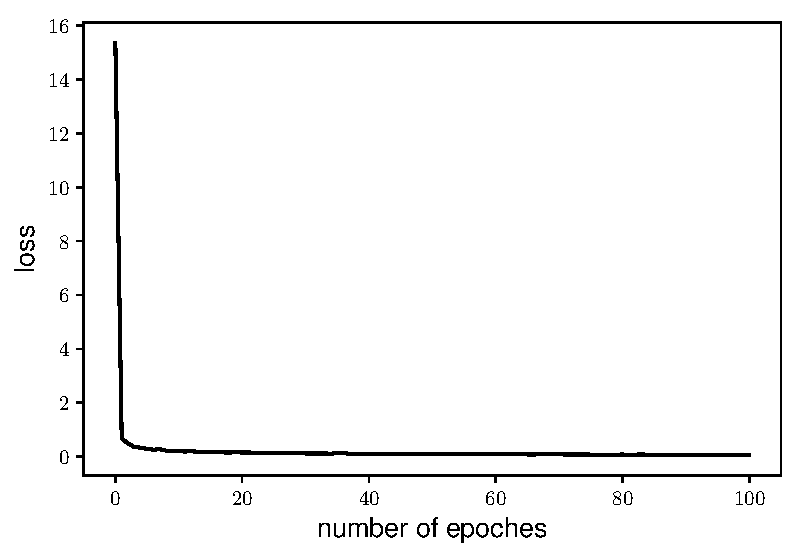
\includegraphics[width=0.99\linewidth]{ebookML_src/src/softmax_regression/softmax_loss.pdf}
    \caption{}
    \label{fig:13_exa}
    \end{subfigure}
    \begin{subfigure}{0.49\textwidth}
    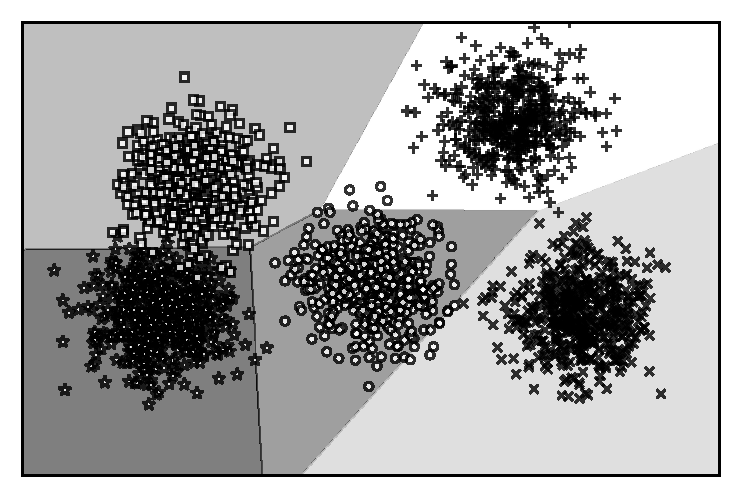
\includegraphics[width=0.99\linewidth]{ebookML_src/src/softmax_regression/softmax_5class.pdf}
    \caption{}
    \label{fig:13_exb}
    \end{subfigure}
    \caption{
    Ví dụ về sử dụng hồi quy softmax cho năm lớp dữ liệu. (a) Giá trị hàm mất mát qua các
    epoch. (b) Kết quả phân loại cuối cùng. 
    }
    \label{fig:13_ex}
\end{figure}
Giá trị của hàm mất mát qua các epoch được cho trên Hình~\ref{fig:13_exa}. Ta
thấy rằng hàm mất mát giảm rất nhanh sau đó hội tụ. Các điểm dữ liệu huấn luyện
của mỗi lớp là các điểm có hình dạng khác nhau trong Hình~\ref{fig:13_exb}. Các
phần có nền khác nhau thể hiện vùng của mỗi lớp dữ liệu tìm được bằng hồi quy
softmax. Ta thấy rằng các đường ranh giới có dạng đường thẳng. Kết quả phân chia
vùng cũng khá tốt, chỉ có một số ít điểm trong tập huấn luyện bị phân loại sai.
Ta cũng thấy hồi quy softmax tốt hơn rất nhiều so với phương pháp kết hợp các bộ
phân loại nhị phân.

%% *****************************************************************************

% Giả sử rằng chúng ta sử dụng mini-batch gradient descent, công thức cập nhật
% cho ma trận trọng số $\bW$ sẽ là
% \begin{equation} 
% \bW = \bW +\eta \mathbf{}_{i}(\mathbf{y}_i - \mathbf{a}_i)^T 
% \end{equation} 

 
% Bạn có thấy công thức này giống với \href{http://machinelearningcoban.com/2017/01/27/logisticregression/#cong-thuc-cap-nhat-cho-logistic-sigmoid-regression}{công thức cập nhật của Logistic Regression} không! 
 
% Thực ra: 
 
 
% \section{Một vài lưu ý khi lập trình với Python }
 
 
% \subsection{Bắt đầu với dữ liệu nhỏ}
% Các bài toán Machine Learning thường có độ phức tạp cao với lượng dữ liệu lớn và nhiều chiều. Để có thể áp dụng một thuật toán vào một bài toán cụ thể, trước tiên chúng ta cần áp dụng thuật toán đó vào \textit{simulated data} (dữ liệu giả) với số chiều và số điểm dữ liệu nhỏ hơn. \textit{Simulated data} này thường được tạo ngẫu nhiên (có thể thêm vài ràng buộc tùy vào đặc thù của dữ liệu). Với \textit{simulated data} nhỏ, chúng ta có thể debug nhanh hơn và thử với nhiều trường hợp \textit{simulated data} khác nhau. Khi nào thấy thuật toán chạy đúng chúng ta mới đưa \textit{dữ liệu thật} vào.  
 
% Với Softmax Regression, tôi tạo \textit{simulated data} như sau:  
 
% \begin{lstlisting}[language=Python]
% import numpy as np  
 
% # randomly generate data  
% N = 2 # number of training sample  
% d = 2 # data dimension  
% C = 3 # number of classes  
 
% X = np.random.randn(d, N) 
% y = np.random.randint(0, 3, (N,)) 
% \end{lstlisting}
% Trong ví dụ đơn giản này, số điểm dữ liệu chỉ là \pythoninline{N = 2}, số chiều dữ liệu \pythoninline{d = 2}, và số classes \pythoninline{C = 3}. Những giá trị đủ nhỏ này giúp cho việc kiểm tra có thể được thực hiện một cách tức thì. Sau khi thuật toán chạy đúng với những giá trị nhỏ này, ta có thể thay \pythoninline{N, d, C} bằng vài giá trị khác trước khi sử dụng dữ liệu thật.  
 
 
% \subsection{Ma trận one-hot coding }
% Có một bước quan trọng nữa trong Softmax Regression là phải chuyển đổi mỗi label $y_i$ thành một vector $\mathbf{y}_i$ dưới dạng one-hot coding. Trong đó, chỉ có đúng một phần tử của $\mathbf{y}_i$ bằng 1, các phần tử còn lại bằng 0. Như vậy, với $N$ điểm dữ liệu và $C$ classes, chúng ta sẽ có một ma trận có kích thước $C \times N$ trong đó mỗi cột chỉ có đúng 1 phần tử bằng 1, còn lại bằng 0. Nếu chúng ta lưu toàn bộ dữ liệu này thì sẽ bị lãng phí bộ nhớ.  
 
% Một cách thường được sử dụng là lưu ma trận output $\mathbf{Y}$ dưới dạng \textit{sparse matrix}. Về cơ bản, cách làm này chỉ lưu các \textbf{vị trí} khác 0 của ma trận và \textbf{giá trị} khác 0 đó.  
 
% Python có hàm \href{https://docs.scipy.org/doc/scipy/reference/generated/scipy.sparse.coo_matrix.html}{\pythoninline{scipy.sparse.coo\_matrix}} giúp chúng ta thực hiện việc này. Với one-hot coding, tôi thực hiện như sau:  
 
% \begin{lstlisting}[language=Python]
% ## One-hot coding 
% from scipy import sparse  
% def convert_labels(y, C = C): 
%     """ 
%     convert 1d label to a matrix label: each column of this  
%     matrix coresponding to 1 element in y. In i-th column of Y,  
%     only one non-zeros element located in the y[i]-th position,  
%     and = 1 ex: y = [0, 2, 1, 0], and 3 classes then return 
 
%             [[1, 0, 0, 1], 
%              [0, 0, 1, 0], 
%              [0, 1, 0, 0]] 
%     """ 
%     Y = sparse.coo_matrix((np.ones_like(y),  
%         (y, np.arange(len(y)))), shape = (C, len(y))).toarray() 
%     return Y  
 
% Y = convert_labels(y, C) 
% \end{lstlisting}
 
 
 
 
% \subsection{Kiểm tra đạo hàm }
% Điều cốt lõi trong cách tối ưu hàm mất mát là tính gradient. Với biểu thức toán trông \textit{khá rối mắt} như trên, rất dễ để các bạn nhầm lẫn ở một bước nào đó. Softmax Regression vẫn là một thuật toán đơn giản, sau này các bạn sẽ thấy nhưng biểu thức phức tạp hơn nhiều. Rất khó để có thể tính toán đúng gradient ở ngay lần thử đầu tiên.  
 
% Trong thực nghiệm, một cách thường được làm là so sánh gradient tính được với \textit{numeric gradient}, tức gradient tính theo định nghĩa. Bạn đọc được khuyến khích đọc cách \href{http://machinelearningcoban.com/2017/01/12/gradientdescent/#kiem-tra-dao-ham}{Kiểm tra đạo hàm}.  
 
% Việc kiểm tra đạo hàm được thực hiện như sau:  
 
% \begin{lstlisting}[language=Python]
% # cost or loss function   
% def cost(X, Y, W): 
%     A = softmax(W.T.dot(X)) 
%     return -np.sum(Y*np.log(A)) 
 
% W_init = np.random.randn(d, C) 
 
% def grad(X, Y, W): 
%     A = softmax((W.T.dot(X))) 
%     E = A - Y 
%     return X.dot(E.T) 
     
% def numerical_grad(X, Y, W, cost): 
%     eps = 1e-6 
%     g = np.zeros_like(W) 
%     for i in range(W.shape[0]): 
%         for j in range(W.shape[1]): 
%             W_p = W.copy() 
%             W_n = W.copy() 
%             W_p[i, j] += eps  
%             W_n[i, j] -= eps 
%             g[i,j] = (cost(X, Y, W_p) - cost(X, Y, W_n))/(2*eps) 
%     return g  
 
% g1 = grad(X, Y, W_init) 
% g2 = numerical_grad(X, Y, W_init, cost) 
 
% print(np.linalg.norm(g1 - g2)) 
% \end{lstlisting}
% Kết quả:
% \begin{lstlisting}
%     2.70479295591e-10 
% \end{lstlisting}
 
 
% Như vậy, sự khác biệt giữa hai đạo hàm là rất nhỏ. Nếu các bạn thử vài trường hợp khác nữa của \pythoninline{N, C, d}, chúng ta sẽ thấy sự sai khác vẫn là nhỏ. Điều này chứng tỏ đạo hàm chúng ta tính được coi là chính xác. (Vẫn có thể có bug, chỉ khi nào kết quả cuối cùng với dữ liệu thật là chấp nhận được thì ta mới có thể bỏ cụm từ 'có thể coi' đi). 
 
% Chú ý rằng, nếu \pythoninline{N, C, d} quá lớn, việc tính toán \pythoninline{numerical_grad} trở nên cực kỳ tốn thời gian và bộ nhớ. Chúng ta chỉ nên kiểm tra với những dữ liệu nhỏ. 
 
% \subsection{Hàm chính cho training Softmax Regression}
 
% Sau khi đã có những hàm cần thiết và gradient được tính đúng, chúng ta có thể viết hàm chính có training Softmax Regression (theo SGD) như sau: 
 
% \begin{lstlisting}[language=Python]
% def softmax_regression(X, y, W_init, eta, tol = 1e-4, max_count = 10000): 
%     W = [W_init]     
%     C = W_init.shape[1] 
%     Y = convert_labels(y, C) 
%     it = 0 
%     N = X.shape[1] 
%     d = X.shape[0] 
     
%     count = 0 
%     check_w_after = 20 
%     while count < max_count: 
%         # mix data  
%         mix_id = np.random.permutation(N) 
%         for i in mix_id: 
%             xi = X[:, i].reshape(d, 1) 
%             yi = Y[:, i].reshape(C, 1) 
%             ai = softmax(np.dot(W[-1].T, xi)) 
%             W_new = W[-1] + eta*xi.dot((yi - ai).T) 
%             count += 1 
%             # stopping criteria 
%             if count%check_w_after == 0:                 
%                 if np.linalg.norm(W_new - W[-check_w_after]) < tol: 
%                     return W 
%             W.append(W_new) 
%     return W 
% eta = .05  
% d = X.shape[0] 
% W_init = np.random.randn(d, C) 
 
% W = softmax_regression(X, y, W_init, eta) 
% # W[-1] is the solution, W is all history of weights 
% \end{lstlisting}
 
 
% \subsection{Hàm dự đoán class cho dữ liệu mới }
 
% Sau khi train Softmax Regression và tính được ma trận hệ số \pythoninline{W}, class của một dữ liệu mới có thể tìm được bằng cách xác định vị trí của giá trị lớn nhất ở đầu ra dự đoán (tương ứng với xác suất điểm dữ liệu rơi vào class đó là lớn nhất). Chú ý rằng, các class được đánh số là \pythoninline{0, 1, 2, ..., C}.  
 
% \begin{lstlisting}[language=Python]
% def pred(W, X): 
%     """ 
%     predict output of each columns of X 
%     Class of each x_i is determined by location of max probability 
%     Note that class are indexed by [0, 1, 2, ...., C-1] 
%     """ 
%     A = softmax_stable(W.T.dot(X)) 
%     return np.argmax(A, axis = 0) 
% \end{lstlisting}
 
 
% \section{Ví dụ với Python}
 
% \subsection{Simulated data}
% Để minh họa cách áp dụng Softmax Regression, tôi tiếp tục làm trên \textit{simulated data}.  
 
% \textbf{Tạo ba cụm dữ liệu} 
% \begin{lstlisting}[language=Python]
% means = [[2, 2], [8, 3], [3, 6]] 
% cov = [[1, 0], [0, 1]] 
% N = 500 
% X0 = np.random.multivariate_normal(means[0], cov, N) 
% X1 = np.random.multivariate_normal(means[1], cov, N) 
% X2 = np.random.multivariate_normal(means[2], cov, N) 
 
% # each column is a datapoint 
% X = np.concatenate((X0, X1, X2), axis = 0).T  
% # extended data 
% X = np.concatenate((np.ones((1, 3*N)), X), axis = 0) 
% C = 3 
 
% original_label = np.asarray([0]*N + [1]*N + [2]*N).T 
% \end{lstlisting}
% Phân bố của các dữ liệu được cho như hình dưới: 
 
% % <div class="imgcap"> 
% % <img src ="\assets\13_softmax\ex1_1.png" align = "center" width = "500"> 
% % <div class = "thecap">Hình 5: Phân bố dữ liệu của các class.</div> 
% % </div> 
% \begin{figure}[t]
%      % caption on side     
%      \floatbox[{\capbeside\thisfloatsetup{capbesideposition={right,top},capbesidewidth=6cm}}]{figure}[\FBwidth]
%      {\caption{ 
%       Phân bố dữ liệu của các lớp.
%      }
%      \label{fig:13_5}}
%      { % figure here
%      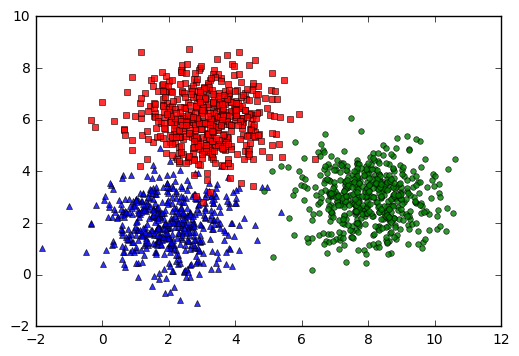
\includegraphics[width=.5\textwidth]{Chapters/05_NeuralNetworks/13_softmax/ex1_1.png}
%      }
%  \end{figure}

 
% \textbf{Thực hiện Softmax Regression} 
 
% \begin{lstlisting}[language=Python]
% W_init = np.random.randn(X.shape[0], C) 
% W = softmax_regression(X, original_label, W_init, eta) 
% print(W[-1]) 
% \end{lstlisting}
% Kết quả:
% \begin{lstlisting}
%     [[ 8.45809734 -3.88415491 -3.44660294] 
%      [-1.11205751  1.50441603 -0.76358758] 
%      [ 0.24484886  0.26085383  3.3658872 ]] 
% \end{lstlisting}
 
% \textbf{Kết quả thu được} được biểu diễn trong Hình \ref{fig:13_6}. 
 
% % <div class="imgcap"> 
% % <img src ="\assets\13_softmax\ex1_2.png" align = "center" width = "500"> 
% % <div class = "thecap">Hình 6: Ranh giới giữa các class tìm được bằng Softmax Regression. </div> 
% % </div>  
% \begin{figure}[t]
%     % caption on side     
%     \floatbox[{\capbeside\thisfloatsetup{capbesideposition={right,top},capbesidewidth=6cm}}]{figure}[\FBwidth]
%     {\caption{ 
%     Đường ranh giới giữa các lớp tìm được bằng Softmax Regression.
%     }
%     \label{fig:13_6}}
%     { % figure here
%     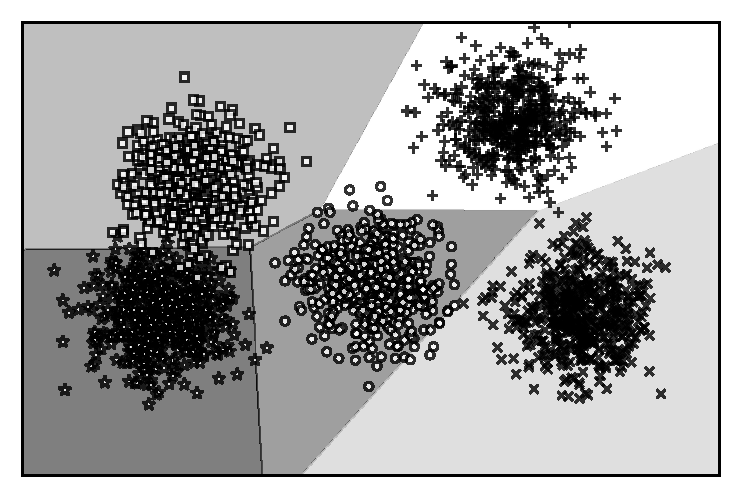
\includegraphics[width=.5\textwidth]{ebookML_src/src/softmax_regression/softmax_5class.pdf}
%     }
% \end{figure}

% Ta thấy rằng Softmax Regression đã tạo ra các vùng cho mỗi class. Kết quả này là chấp nhận được. Từ hình trên ta cũng thấy rằng \textit{đường ranh giới} giữa các classes là đường thẳng. Tôi sẽ chứng minh điều này ở phần sau.  
 
 
% \subsection{Softmax Regression cho MNIST}
\newpage 
\textbf{MNIST với hồi quy softmax trong scikit-learn}

% Các ví dụ trên đây được trình bày để giúp bạn đọc hiểu rõ Softmax Regression hoạt động như thế nào. Khi làm việc với các bài toán thực tế, chúng ta nên sử dụng các thư viện có sẵn, trừ khi bạn có thêm bớt vài số hạng nữa trong hàm mất mat.  
Trong scikit-learn, hồi quy softmax được tích hợp trong class
\pythoninline{sklearn.linear_model.LogisticRegression}. Như sẽ thấy trong phần
thảo luận, hồi quy logistic chính là hồi quy softmax cho bài toán phân loại nhị
phân. Với bài toán phân loại đa lớp, thư viện này mặc định sử dụng kỹ thuật
one-vs-rest. Để sử dụng hồi quy softmax, ta thay đổi thuộc tính
\pythoninline{multi_class = 'multinomial'} và \pythoninline{solver = 'lbfgs'}.
Ở đây, \pythoninline{'lbfgs'} là một phương pháp tối ưu rất mạnh cũng dựa trên
gradient. Trong khuôn khổ của cuốn sách, chúng ta sẽ không thảo luận về phương
pháp này\footnote{Đọc thêm: \textit{Limited-memory BFGS -- Wikipedia} (\url{https://goo.gl/qf1kmn}).}. 

Quay lại với bài toán phân loại chữ số viết tay trong cơ sở dữ liệu MNIST. Đoạn
code dưới đây thực hiện việc lấy ra 10000 điểm dữ liệu trong số 70000 điểm làm
tập kiểm tra, còn lại là tập huấn luyện. Bộ phân loại được sử dụng là hồi quy softmax.
% \newpage 

% Softmax Regression cũng được tích hợp trong hàm \href{http://scikit-learn.org/stable/modules/generated/sklearn.linear_model.LogisticRegression.html}{\pythoninline{sklearn.linear\_model.LogisticRegression}} của thư viện \href{http://scikit-learn.org/stable/index.html}{sklearn}.  
 
% Để sử dụng Softmax Regression, ta cần thêm một vài thuộc tính nữa:  
% \begin{lstlisting}[language=Python]
% linear_model.LogisticRegression(C=1e5, solver = 'lbfgs', multi_class = 'multinomial') 
% \end{lstlisting}
 
% Với Logistic Regression, \pythoninline{multi_class = 'ovr'} là giá trị mặc định, tương ứng với \textbf{one-vs-rest}. \pythoninline{solver = 'lbfgs'} là một phương pháp tối ưu cũng dựa trên gradient nhưng hiệu quả hơn và phức tạp hơn Gradient Descent. Bạn đọc có thể \href{https://en.wikipedia.org/wiki/Limited-memory_BFGS}{đọc thêm ở đây}.  
 
\begin{lstlisting}[language=Python]
import numpy as np 
from sklearn.datasets import fetch_mldata
from sklearn.linear_model import LogisticRegression 
from sklearn.model_selection import train_test_split
from sklearn.metrics import accuracy_score
mnist = fetch_mldata('MNIST original', data_home='../../data/')

X = mnist.data 
y = mnist.target
X_train, X_test, y_train, y_test = train_test_split(X, y, test_size=10000)

model = LogisticRegression(C = 1e5,
        solver = 'lbfgs', multi_class = 'multinomial') # C is inverse of lam 
model.fit(X_train, y_train)

y_pred = model.predict(X_test)
print("Accuracy %.2f %%" % (100*accuracy_score(y_test, y_pred.tolist())))
\end{lstlisting}
Kết quả:
\begin{lstlisting}
    Accuracy: 92.19 % 
\end{lstlisting}
 
So với kết quả hơn 91.7\% của one-vs-rest hồi quy logistic, kết quả
của hồi quy softmax đã được cải thiện. Kết quả thấp này hoàn toàn có thể dự đoán được vì thực ra hồi quy softmax chỉ tạo ra các đường
ranh giới tuyến tính. Kết quả tốt nhất của bài toán phân loại chữ
số trong MNIST hiện nay vào khoảng hơn 99.7\%, đạt được bằng một mạng neuron tích chập với rất nhiều tầng ẩn và tầng cuối cùng là một
hồi quy softmax. 
 
 
\section{Thảo luận }
 
\subsection{Hồi quy logistic là trường hợp đặc biệt của hồi quy softmax}
 
Khi $C = 2$, hồi quy softmax và hồi quy logistic là hai mô hình giống nhau. Thật vậy,
với $C = 2$, đầu ra của hàm softmax cho một đầu vào $\bx$ là:
\begin{equation}
    a_1 = \frac{\exp(\bx^T\bw_1)} {\exp(\bx^T\bw_1) +
\exp(\bx^T\bw_2)} 
= \frac{1}{1 + \exp(\bx^T(\bw_2 - \bw_1))};\quad a_2 = 1 -
a_1
\end{equation}
Từ đây ta thấy rằng, $a_1$ có dạng là một hàm sigmoid với vector trọng số có dạng $\bw =
-(\bw_2 - \bw_1)$.
Khi $C = 2$, bạn đọc cũng có thể thấy rằng hàm mất mát của hồi quy logistic
và hồi quy softmax là như nhau. Hơn nữa, mặc dù có hai đầu ra, hồi quy softmax có thể biểu diễn bởi một đầu ra vì tổng của chúng bằng một.

% một đầu ra dự đoán của hồi quy softmax với $C= 2$ có thể được viết dưới
% dạng
% \begin{equation} 
% a_1 = \frac{\exp(\bx^T\bw_1)} {\exp(\bx^T\bw_1) +
% \exp(\bw_2^T\bx)} 
% = \frac{1}{1 + \exp((\bw_2 - \bw_1)^T\bx)} 
% \end{equation} 
% Đây chính là \href{http://machinelearningcoban.com/2017/01/27/logisticregression/#sigmoid-function}{sigmoid function}, là đầu ra dự đoán theo Logistic Regression. 
\index{hồi quy logistic multinomial}
% \index{maximum entropy classifier}
 {Giống như hồi quy logistic, hồi quy softmax được sử dụng trong các bài toán
phân loại}. Các tên gọi này được giữ lại vì vấn đề lịch sử.

 % Xem thêm \href{https://en.wikipedia.org/wiki/Multinomial_logistic_regression}
 % {Multinomial hồi quy logistic - Wikipedia}
 
\subsection{Ranh giới tạo bởi hồi quy softmax là các mặt tuyến tính}
Thật vậy, dựa vào hàm softmax thì một điểm dữ liệu $\bx$ được dự đoán là rơi vào class $j$ nếu $a_{j} \geq a_{k}, ~\forall k \neq j$. Bạn đọc có thể chứng minh được rằng:
% $a_{j} \geq a_{k} \Leftrightarrow z_{j} \geq z_{k}$, hay nói cách khác:  
\begin{equation} 
a_{j} \geq a_{k} \Leftrightarrow z_{j} \geq z_{k} \Leftrightarrow \bx^T\bw_j \geq \bx^T\bw_k\\\
\Leftrightarrow \bx^T(\bw_j - \bw_k) \geq 0.
\end{equation} 
Như vậy, một điểm thuộc lớp thứ $j$ nếu và chỉ nếu $\bx^T(\bw_j - \bw_k) \geq
0,~\forall k \neq j$. Như vậy, mỗi lớp dữ liệu chiếm một vùng là giao
của các nửa không gian. Nói cách khác, đường ranh giới giữa các lớp là các
mặt tuyến tính. 
% Đây chính là một biểu thức tuyến tính. Vậy boundary tạo bởi Softmax Regression có dạng tuyến tính. (Xem thêm \href{http://machinelearningcoban.com/2017/01/27/logisticregression/#boundary-tao-boi-logistic-regression-co-dang-tuyen-tinh}{boundary tạo bởi Logistic Regression})  
 
 
\subsection{Hồi quy softmax là một trong hai bộ phân loại phổ biến nhất}
Hồi quy softmax cùng với máy vector hỗ trợ đa lớp
(Chương~\ref{cha:multisvm}) là hai bộ phân loại phổ biến nhất được dùng hiện nay.
Hồi quy softmax đặc biệt được sử dụng nhiều trong các mạng neuron sâu với
rất nhiều tầng ẩn. Những tầng phía trước có thể được coi như một bộ trích chọn 
vector đặc trưng, tầng cuối cùng thường là một hồi quy softmax.
 
 
Mã nguồn của chương này có thể được tìm thấy tại \url{https://goo.gl/XU8ZXm}.
 % \section{Tài liệu tham khảo }
% [1] \href{http://ufldl.stanford.edu/tutorial/supervised/SoftmaxRegression/}{Softmax Regression} 
 
% [2] \href{http://scikit-learn.org/stable/modules/generated/sklearn.linear_model.LogisticRegression.html}{\pythoninline{sklearn.linear\_model.LogisticRegression}} 
 
% [3] \href{https://en.wikipedia.org/wiki/Softmax_function}{Softmax function - Wikipedia} 
 
% [4] \href{http://neuralnetworksanddeeplearning.com/chap3.html}{Improving the way neural networks learn} 
 
